\documentclass[12pt]{article}
%Fall 2022
% Some basic packages
\usepackage{standalone}[subpreambles=true]
\usepackage[utf8]{inputenc}
\usepackage[T1]{fontenc}
\usepackage{textcomp}
\usepackage[english]{babel}
\usepackage{url}
\usepackage{graphicx}
%\usepackage{quiver}
\usepackage{float}
\usepackage{enumitem}
\usepackage{lmodern}
\usepackage{comment}
\usepackage{hyperref}
\usepackage[usenames,svgnames,dvipsnames]{xcolor}
\usepackage[margin=1in]{geometry}
\usepackage{pdfpages}

\pdfminorversion=7

% Don't indent paragraphs, leave some space between them
\usepackage{parskip}

% Hide page number when page is empty
\usepackage{emptypage}
\usepackage{subcaption}
\usepackage{multicol}
\usepackage[b]{esvect}

% Math stuff
\usepackage{amsmath, amsfonts, mathtools, amsthm, amssymb}
\usepackage{bbm}
\usepackage{stmaryrd}
\allowdisplaybreaks

% Fancy script capitals
\usepackage{mathrsfs}
\usepackage{cancel}
% Bold math
\usepackage{bm}
% Some shortcuts
\newcommand{\rr}{\ensuremath{\mathbb{R}}}
\newcommand{\zz}{\ensuremath{\mathbb{Z}}}
\newcommand{\qq}{\ensuremath{\mathbb{Q}}}
\newcommand{\nn}{\ensuremath{\mathbb{N}}}
\newcommand{\ff}{\ensuremath{\mathbb{F}}}
\newcommand{\cc}{\ensuremath{\mathbb{C}}}
\newcommand{\ee}{\ensuremath{\mathbb{E}}}
\newcommand{\hh}{\ensuremath{\mathbb{H}}}
\renewcommand\O{\ensuremath{\emptyset}}
\newcommand{\norm}[1]{{\left\lVert{#1}\right\rVert}}
\newcommand{\dbracket}[1]{{\left\llbracket{#1}\right\rrbracket}}
\newcommand{\ve}[1]{{\bm{#1}}}
\newcommand\allbold[1]{{\boldmath\textbf{#1}}}
\DeclareMathOperator{\lcm}{lcm}
\DeclareMathOperator{\im}{im}
\DeclareMathOperator{\coim}{coim}
\DeclareMathOperator{\dom}{dom}
\DeclareMathOperator{\tr}{tr}
\DeclareMathOperator{\rank}{rank}
\DeclareMathOperator*{\var}{Var}
\DeclareMathOperator*{\ev}{E}
\DeclareMathOperator{\dg}{deg}
\DeclareMathOperator{\aff}{aff}
\DeclareMathOperator{\conv}{conv}
\DeclareMathOperator{\inte}{int}
\DeclareMathOperator*{\argmin}{argmin}
\DeclareMathOperator*{\argmax}{argmax}
\DeclareMathOperator{\graph}{graph}
\DeclareMathOperator{\sgn}{sgn}
\DeclareMathOperator*{\Rep}{Rep}
\DeclareMathOperator{\Proj}{Proj}
\DeclareMathOperator{\mat}{mat}
\DeclareMathOperator{\diag}{diag}
\DeclareMathOperator{\aut}{Aut}
\DeclareMathOperator{\gal}{Gal}
\DeclareMathOperator{\inn}{Inn}
\DeclareMathOperator{\edm}{End}
\DeclareMathOperator{\Hom}{Hom}
\DeclareMathOperator{\ext}{Ext}
\DeclareMathOperator{\tor}{Tor}
\DeclareMathOperator{\Span}{Span}
\DeclareMathOperator{\Stab}{Stab}
\DeclareMathOperator{\cont}{cont}
\DeclareMathOperator{\Ann}{Ann}
\DeclareMathOperator{\Div}{div}
\DeclareMathOperator{\curl}{curl}
\DeclareMathOperator{\nat}{Nat}
\DeclareMathOperator{\gr}{Gr}
\DeclareMathOperator{\vect}{Vect}
\DeclareMathOperator{\id}{id}
\DeclareMathOperator{\Mod}{Mod}
\DeclareMathOperator{\sign}{sign}
\DeclareMathOperator{\Surf}{Surf}
\DeclareMathOperator{\fcone}{fcone}
\DeclareMathOperator{\Rot}{Rot}
\DeclareMathOperator{\grad}{grad}
\DeclareMathOperator{\atan2}{atan2}
\DeclareMathOperator{\Ric}{Ric}
\let\vec\relax
\DeclareMathOperator{\vec}{vec}
\let\Re\relax
\DeclareMathOperator{\Re}{Re}
\let\Im\relax
\DeclareMathOperator{\Im}{Im}
% Put x \to \infty below \lim
\let\svlim\lim\def\lim{\svlim\limits}

%wide hat
\usepackage{scalerel,stackengine}
\stackMath
\newcommand*\wh[1]{%
\savestack{\tmpbox}{\stretchto{%
  \scaleto{%
    \scalerel*[\widthof{\ensuremath{#1}}]{\kern-.6pt\bigwedge\kern-.6pt}%
    {\rule[-\textheight/2]{1ex}{\textheight}}%WIDTH-LIMITED BIG WEDGE
  }{\textheight}% 
}{0.5ex}}%
\stackon[1pt]{#1}{\tmpbox}%
}
\parskip 1ex

%Make implies and impliedby shorter
\let\implies\Rightarrow
\let\impliedby\Leftarrow
\let\iff\Leftrightarrow
\let\epsilon\varepsilon

% Add \contra symbol to denote contradiction
\usepackage{stmaryrd} % for \lightning
\newcommand\contra{\scalebox{1.5}{$\lightning$}}

% \let\phi\varphi

% Command for short corrections
% Usage: 1+1=\correct{3}{2}

\definecolor{correct}{HTML}{009900}
\newcommand\correct[2]{\ensuremath{\:}{\color{red}{#1}}\ensuremath{\to }{\color{correct}{#2}}\ensuremath{\:}}
\newcommand\green[1]{{\color{correct}{#1}}}

% horizontal rule
\newcommand\hr{
    \noindent\rule[0.5ex]{\linewidth}{0.5pt}
}

% hide parts
\newcommand\hide[1]{}

% si unitx
\usepackage{siunitx}
\sisetup{locale = FR}

%allows pmatrix to stretch
\makeatletter
\renewcommand*\env@matrix[1][\arraystretch]{%
  \edef\arraystretch{#1}%
  \hskip -\arraycolsep
  \let\@ifnextchar\new@ifnextchar
  \array{*\c@MaxMatrixCols c}}
\makeatother

\renewcommand{\arraystretch}{0.8}

\renewcommand{\baselinestretch}{1.5}

\usepackage{graphics}
\usepackage{epstopdf}

\RequirePackage{hyperref}
%%
%% Add support for color in order to color the hyperlinks.
%% 
\hypersetup{
  colorlinks = true,
  urlcolor = blue,
  citecolor = blue
}
%%fakesection Links
\hypersetup{
    colorlinks,
    linkcolor={red!50!black},
    citecolor={green!50!black},
    urlcolor={blue!80!black}
}
%customization of cleveref
\RequirePackage[capitalize,nameinlink]{cleveref}[0.19]

% Per SIAM Style Manual, "section" should be lowercase
\crefname{section}{section}{sections}
\crefname{subsection}{subsection}{subsections}
\Crefname{section}{Section}{Sections}
\Crefname{subsection}{Subsection}{Subsections}

% Per SIAM Style Manual, "Figure" should be spelled out in references
\Crefname{figure}{Figure}{Figures}

% Per SIAM Style Manual, don't say equation in front on an equation.
\crefformat{equation}{\textup{#2(#1)#3}}
\crefrangeformat{equation}{\textup{#3(#1)#4--#5(#2)#6}}
\crefmultiformat{equation}{\textup{#2(#1)#3}}{ and \textup{#2(#1)#3}}
{, \textup{#2(#1)#3}}{, and \textup{#2(#1)#3}}
\crefrangemultiformat{equation}{\textup{#3(#1)#4--#5(#2)#6}}%
{ and \textup{#3(#1)#4--#5(#2)#6}}{, \textup{#3(#1)#4--#5(#2)#6}}{, and \textup{#3(#1)#4--#5(#2)#6}}

% But spell it out at the beginning of a sentence.
\Crefformat{equation}{#2Equation~\textup{(#1)}#3}
\Crefrangeformat{equation}{Equations~\textup{#3(#1)#4--#5(#2)#6}}
\Crefmultiformat{equation}{Equations~\textup{#2(#1)#3}}{ and \textup{#2(#1)#3}}
{, \textup{#2(#1)#3}}{, and \textup{#2(#1)#3}}
\Crefrangemultiformat{equation}{Equations~\textup{#3(#1)#4--#5(#2)#6}}%
{ and \textup{#3(#1)#4--#5(#2)#6}}{, \textup{#3(#1)#4--#5(#2)#6}}{, and \textup{#3(#1)#4--#5(#2)#6}}

% Make number non-italic in any environment.
\crefdefaultlabelformat{#2\textup{#1}#3}

% Environments
\makeatother
% For box around Definition, Theorem, \ldots
%%fakesection Theorems
\usepackage{thmtools}
\usepackage[framemethod=TikZ]{mdframed}

\theoremstyle{definition}
\mdfdefinestyle{mdbluebox}{%
	roundcorner = 10pt,
	linewidth=1pt,
	skipabove=12pt,
	innerbottommargin=9pt,
	skipbelow=2pt,
	nobreak=true,
	linecolor=blue,
	backgroundcolor=TealBlue!5,
}
\declaretheoremstyle[
	headfont=\sffamily\bfseries\color{MidnightBlue},
	mdframed={style=mdbluebox},
	headpunct={\\[3pt]},
	postheadspace={0pt}
]{thmbluebox}

\mdfdefinestyle{mdredbox}{%
	linewidth=0.5pt,
	skipabove=12pt,
	frametitleaboveskip=5pt,
	frametitlebelowskip=0pt,
	skipbelow=2pt,
	frametitlefont=\bfseries,
	innertopmargin=4pt,
	innerbottommargin=8pt,
	nobreak=false,
	linecolor=RawSienna,
	backgroundcolor=Salmon!5,
}
\declaretheoremstyle[
	headfont=\bfseries\color{RawSienna},
	mdframed={style=mdredbox},
	headpunct={\\[3pt]},
	postheadspace={0pt},
]{thmredbox}

\declaretheorem[%
style=thmbluebox,name=Theorem,numberwithin=section]{thm}
\declaretheorem[style=thmbluebox,name=Lemma,sibling=thm]{lem}
\declaretheorem[style=thmbluebox,name=Proposition,sibling=thm]{prop}
\declaretheorem[style=thmbluebox,name=Corollary,sibling=thm]{coro}
\declaretheorem[style=thmredbox,name=Example,sibling=thm]{eg}

\mdfdefinestyle{mdgreenbox}{%
	roundcorner = 10pt,
	linewidth=1pt,
	skipabove=12pt,
	innerbottommargin=9pt,
	skipbelow=2pt,
	nobreak=true,
	linecolor=ForestGreen,
	backgroundcolor=ForestGreen!5,
}

\declaretheoremstyle[
	headfont=\bfseries\sffamily\color{ForestGreen!70!black},
	bodyfont=\normalfont,
	spaceabove=2pt,
	spacebelow=1pt,
	mdframed={style=mdgreenbox},
	headpunct={ --- },
]{thmgreenbox}

\declaretheorem[style=thmgreenbox,name=Definition,sibling=thm]{defn}

\mdfdefinestyle{mdgreenboxsq}{%
	linewidth=1pt,
	skipabove=12pt,
	innerbottommargin=9pt,
	skipbelow=2pt,
	nobreak=true,
	linecolor=ForestGreen,
	backgroundcolor=ForestGreen!5,
}
\declaretheoremstyle[
	headfont=\bfseries\sffamily\color{ForestGreen!70!black},
	bodyfont=\normalfont,
	spaceabove=2pt,
	spacebelow=1pt,
	mdframed={style=mdgreenboxsq},
	headpunct={},
]{thmgreenboxsq}
\declaretheoremstyle[
	headfont=\bfseries\sffamily\color{ForestGreen!70!black},
	bodyfont=\normalfont,
	spaceabove=2pt,
	spacebelow=1pt,
	mdframed={style=mdgreenboxsq},
	headpunct={},
]{thmgreenboxsq*}

\mdfdefinestyle{mdblackbox}{%
	skipabove=8pt,
	linewidth=3pt,
	rightline=false,
	leftline=true,
	topline=false,
	bottomline=false,
	linecolor=black,
	backgroundcolor=RedViolet!5!gray!5,
}
\declaretheoremstyle[
	headfont=\bfseries,
	bodyfont=\normalfont\small,
	spaceabove=0pt,
	spacebelow=0pt,
	mdframed={style=mdblackbox}
]{thmblackbox}

\theoremstyle{plain}
\declaretheorem[name=Question,sibling=thm,style=thmblackbox]{ques}
\declaretheorem[name=Remark,sibling=thm,style=thmgreenboxsq]{remark}
\declaretheorem[name=Remark,sibling=thm,style=thmgreenboxsq*]{remark*}
\newtheorem{ass}[thm]{Assumptions}

\theoremstyle{definition}
\newtheorem*{problem}{Problem}
\newtheorem{claim}[thm]{Claim}
\theoremstyle{remark}
\newtheorem*{case}{Case}
\newtheorem*{notation}{Notation}
\newtheorem*{note}{Note}
\newtheorem*{motivation}{Motivation}
\newtheorem*{intuition}{Intuition}
\newtheorem*{conjecture}{Conjecture}

% Make section starts with 1 for report type
%\renewcommand\thesection{\arabic{section}}

% End example and intermezzo environments with a small diamond (just like proof
% environments end with a small square)
\usepackage{etoolbox}
\AtEndEnvironment{vb}{\null\hfill$\diamond$}%
\AtEndEnvironment{intermezzo}{\null\hfill$\diamond$}%
% \AtEndEnvironment{opmerking}{\null\hfill$\diamond$}%

% Fix some spacing
% http://tex.stackexchange.com/questions/22119/how-can-i-change-the-spacing-before-theorems-with-amsthm
\makeatletter
\def\thm@space@setup{%
  \thm@preskip=\parskip \thm@postskip=0pt
}

% Fix some stuff
% %http://tex.stackexchange.com/questions/76273/multiple-pdfs-with-page-group-included-in-a-single-page-warning
\pdfsuppresswarningpagegroup=1


% My name
\author{Jaden Wang}



\begin{document}
\centerline {\textsf{\textbf{\LARGE{Homework 3}}}}
\centerline {Jaden Wang}
\vspace{.15in}

\begin{problem}[3]
Note that I used $ (x,1) \sim (f(x),0)$ for the problem.

We wish to use SvK (note that it might be easier to figure out via building a CW-complex). Let $ v$ be the wedge point of $ X$, and let $ U_0$ be the thickened $ \{v\} \times I$ which is open. Define $ A = U_0 \cup X \times I \setminus \{\frac{1}{2}\} ,B = X \times \left( \frac{1}{4}, \frac{3}{4} \right) $ as figure shown.
~\begin{figure}[H]
	\centering
	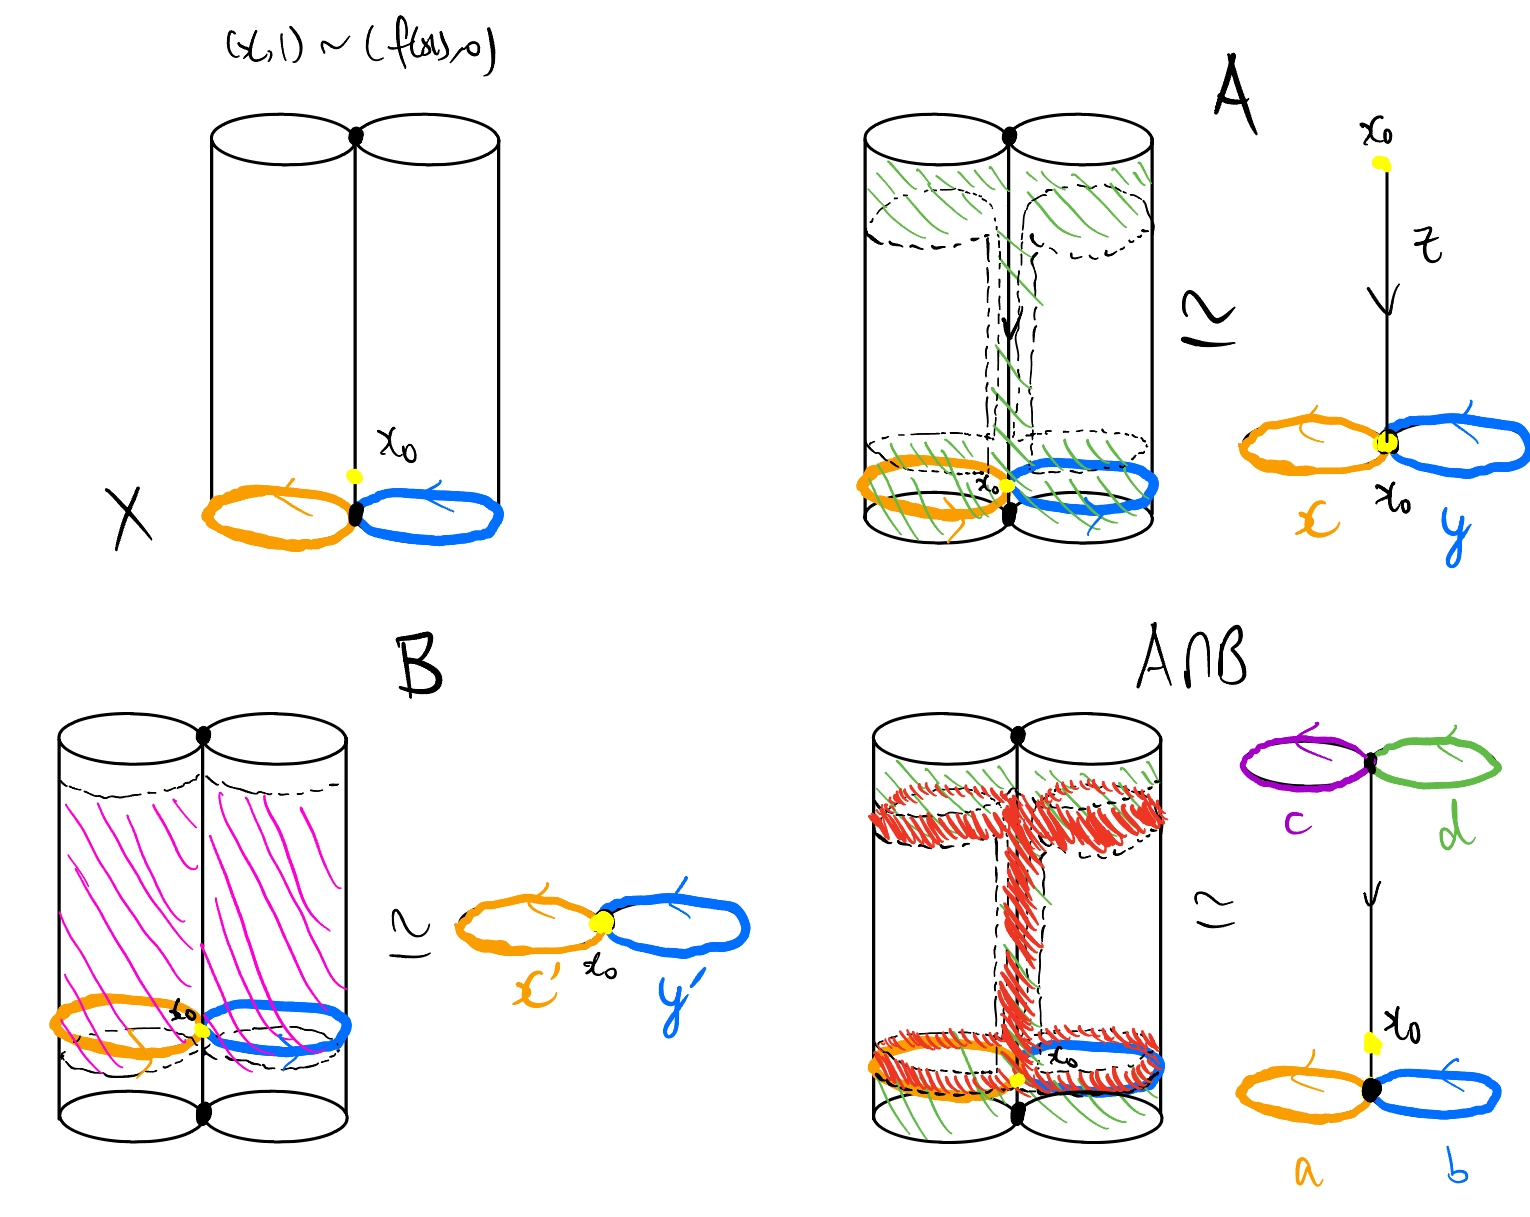
\includegraphics[width=0.8\textwidth]{./figures/svk_mapping_torus.png}
	\caption{We omit the gluing detail at the top but one should keep it}
\end{figure}

Choose the base point $x_0:= \{v\} \times \{\frac{2}{5}\}$ (yellow) so that it is contained in $ A,B,A \cap B$. By pushing the bottom up (so the base becomes $ X \times \{\frac{2}{5}\} $) and applying the identification on the top, \emph{i.e.} we can pretend that $ (f(x),1) \in X \times \{\frac{2}{5}\} $, thus $ A$ has the shown homotopy equivalence. Clearly $ B$ is homotopic to  $ X$ by collapsing the height. Lastly,  $ A \cap B$ is homotopic to a wedge of 4 circles by collapsing to the skeleton. Therefore, we have $ \pi_1( A \cap B) = \langle a,b,c,d| \rangle$, $ \pi_1( A) = \langle x,y,z| \rangle$ and $ \pi_1( B) = \langle x',y'| \rangle$. 

Now let's see what inclusion map induces on the fundamental groups. When we include $ a,b$ in  $ A$, they are precisely $ x,y$ respectively. When we include  $ c,d$ in  $ A$, we push them to the top so they are identified with loops postcomposed with $f$. Note that for $ c,d$ to be expressed by $ x,y$, they must travel down first along  $ z$ in the $ A$ skeleton to get the correct orientation. That is, $ c \mapsto z f_*(x) z^{-1}$ and $ d \mapsto zf_*(y)z^{-1}$. It is clear that for $ A \cap B \to B$ we just map $ a,c \mapsto x',b,d\mapsto y'$. Thus the fibered coproduct is
\begin{align*}
	\pi_1( T_f) &= \langle x,y,z,x',y'|x(x')^{-1},y(y')^{-1},zf_*(x)z^{-1}x', zf_*(y)z^{-1}y' \rangle \\
	&= \langle x,y,z|zf_*(x)z^{-1}x^{-1}, zf_*(y)z^{-1}y^{-1} \rangle .
\end{align*}
\end{problem}

\begin{problem}[6]
~\begin{figure}[H]
	\centering
	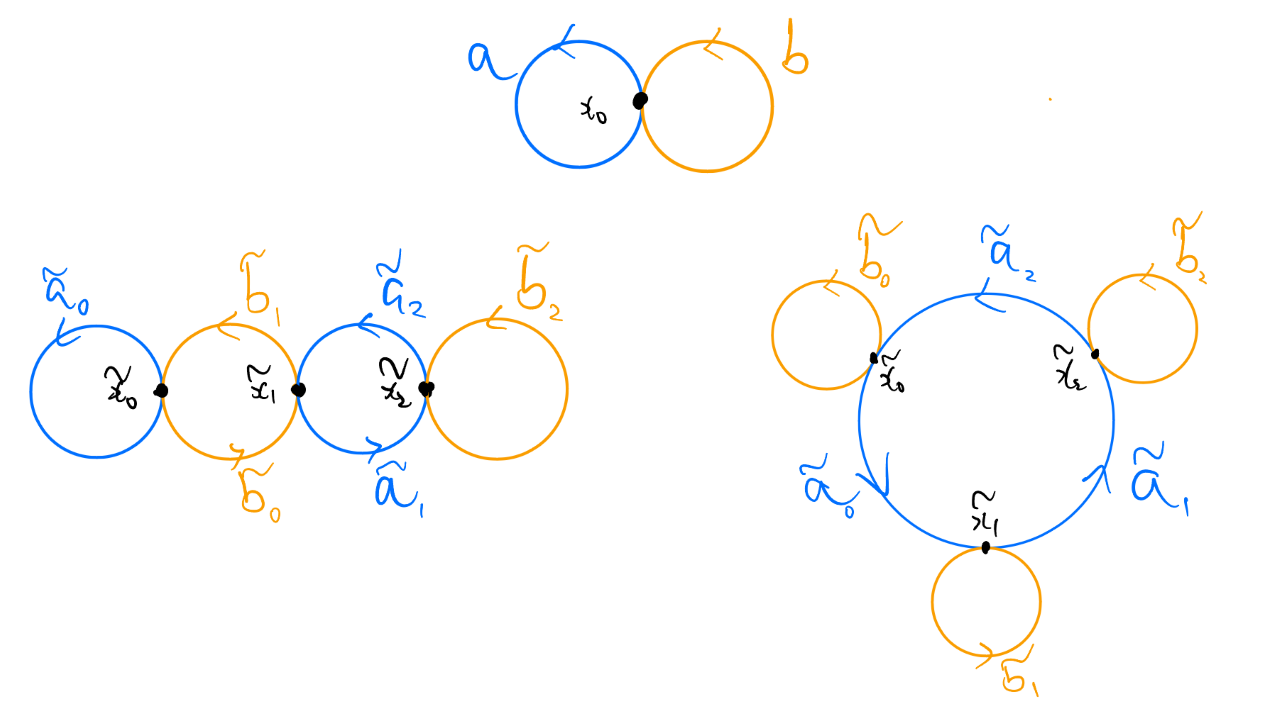
\includegraphics[width=0.8\textwidth]{./figures/normal_cover.png}
	\caption{}
\end{figure}
Since $ \pi_1( S^{1} \vee S^{1}) = \zz*\zz =F_2$, and by the correspondence theorem, index $ n$ subgroups of $ F_2$ corresponds to $ n$-fold covering spaces of  $ S^{1} \vee S^{1}$, it suffices find a normal and non-normal 3-fold covers of $ S^{1} \vee S^{1}$. In the figure, it is straightforward to verify that both are 3-fold covers. The right figure is clearly normal as it has $ \frac{\pi}{ 3}$ rotational symmetry, which is the automorphism that maps between points in $ p^{-1}(x_0)$. It corresponds to a normal subgroup $ N = \langle a,b^2,ba^2b,babab \rangle$. I claim that the left figure is not normal. In particular, there is no deck transformation that maps $ \widetilde{ x}_0$ to $ \widetilde{ x}_1$, since the lift of $ a$ based at  $ \widetilde{ x}_0$ is a loop. and the lift of $ a$ based at  $ \widetilde{ x}_1$ is a path, and they cannot be homeomorphic so no deck transformation sends $ \widetilde{ x}_0$ to $ \widetilde{ x}_1$. It corresponds to $ H = \langle b,a^3,aba^2,a^2ba,ababa \rangle$.
\end{problem}

\begin{problem}[7]
Since $ S^{n}$ is simply connected, any $ f: S^{n} \to X$ satisfies the lifting criterion $ f_*( \pi_1(S^{n})) = p_*(\widetilde{ X}) = 0$. Thus we obtain a lift $ \widetilde{ f}: S^{n} \to X$. Since $ \widetilde{ X}$ is contractible, $ \widetilde{ f}$ is homotopic to the constant map via $ H: S^{n} \times I \to \widetilde{ X}$. As we see from the figure, since $ H(x,1)$ is constant, we can quotient it out to $ H':S^{n} \times I / S^{n} \times \{1\} \to \widetilde{ X}$. The quotient is a cone of $ S^{n}$, clearly homeomorphic to $ D^{n+1}$ with $ \widetilde{ f}$ on the boundary. Denote this modified $ H'$ as  $ \widetilde{ H}: D^{n+1} \to \widetilde{ X}$. Thus we obtain a map $ F:= p \circ \widetilde{ H} : D^{n+1} \to X$, and $ F|_{ \partial D^{n+1}} = p \circ \widetilde{ f} = f$ so it is the extension we seek.
~\begin{figure}[H]
	\centering
	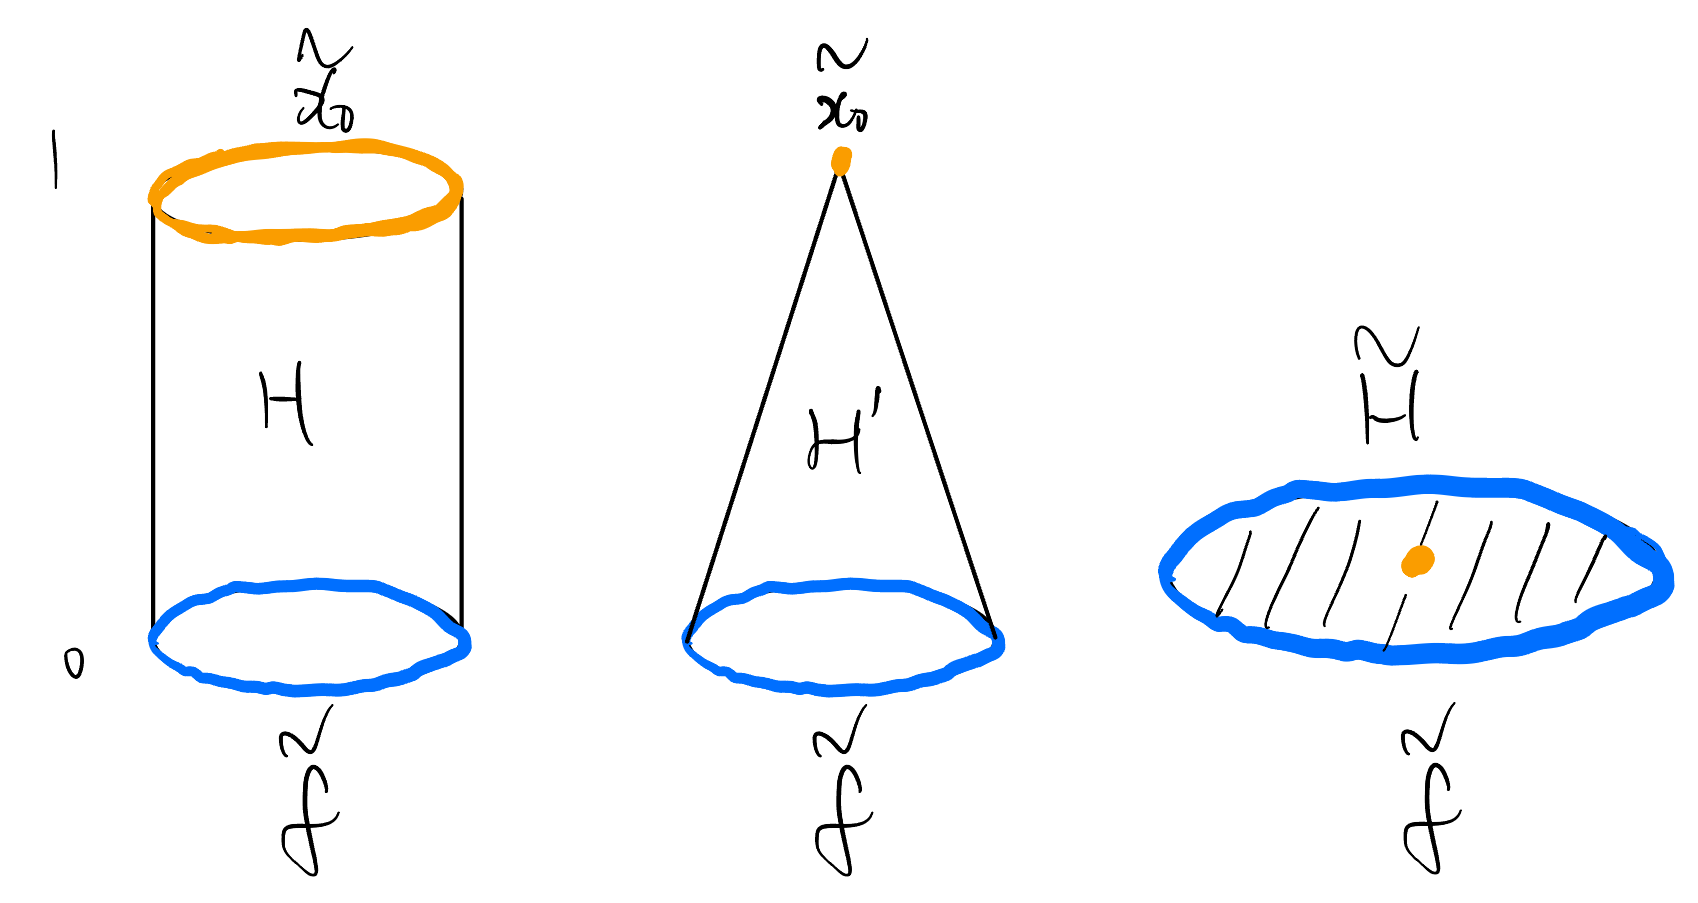
\includegraphics[width=0.8\textwidth]{./figures/extension2.png}
	\caption{}
\end{figure}
\end{problem}

\begin{problem}[8]
	We shall define $ f$ inductively on the skeletons of  $ Y$. Since  $ Y^{(0)}$ is a discrete set of points, define $ f_0 : Y^{(0)} \to X, y \mapsto x_0$, and it is a constant map so it is continuous. Since $ Y$ is path-connected,  $ Y^{(1)}$ must be path-connected too, since the paths between 0-cells must traverse the 1-cells. We can quotient all 0-cells and paths between them so that $ Y^{(1)}$ becomes a wedge of circles. Clearly we can trace out each circle via a loop, $ \gammag$. Then take any representative $ \eta \in \phi([ \gamma]): S^{1} \to X$ and define that to be $ f$ on that circle (think of circle as the quotient of an interval via attaching maps). Doing this for all circles yields a continuous map via the universal property of quotient map map defined for all circles $ f_1: Y^{(1)} \to X$ where $ f_1$ is constant on the 0-cells and 1-cells connecting the 0-cells, so $ f_1$ clearly extends $ f_0$.

	Next, we consider $ Y^{(2)}$, which is obtained from $ Y^{(1)}$ by attaching $ D^2$. Since any attaching map $ a: S^{1} \to Y^{(1)}$ extends to a characteristic map bounding a disk $ D^2 \to Y^{(1)}$, $ D^2$ is contractible and $ Y^{(1)}$ path-connected, $ a$ is nullhomotopic. Since $ a$ introduces a relation in  $ \pi_1( Y) $, there exists some words in $ \pi_1( Y) $ that gets killed. Since $ \phi$ is a homomorphism, we see that $ \phi={f_1}_*$ takes the words to constant as well, making $ f_1 \circ a: S^{1} \to X$ also nullhomotopic. Thus it extends to a map  $ D^2 \to X$, and we are allowed to define $ f_2$ to be this map on the 2-cell using universal property of quotient map. Doing this for all 2-cells yield $ f_2$ that extends $ f_1$. 

	We establish the base case for $ n=2$. Now for induction ($ n\geq 2)$, assume that the desired $ f_n: Y^{(n)} \to X$ is defined. For each $ D^{n+1}$ we attach to $ Y^{(n)}$ via the attaching map $ a: S^{n} \to Y$. Then $ f_n \circ a: S^{n} \to X$ extends to $ g: D^{n+1} \to X$ by Problem 7. Thus we can define a map $ h:=(f_n,g): Y^{(n)} \sqcup D^{n+1} \to X$. Since $ g(x) = f_n(a(x))$ at the gluing site, the map is constant on each equivalent class of $ Y^{(n)} \sqcup_{a} D^{n+1}$ so we obtain a continuous map $ h':Y^{(n)} \sqcup_a D^{n+1} \to X$. Constructing such map for all $ (n+1)$-cells simultaneously yields a map  $ f_{n+1}: Y^{(n+1)} \to X$, completing the inductive step.
\end{problem}

\begin{problem}[11]
~\begin{figure}[H]
	\centering
	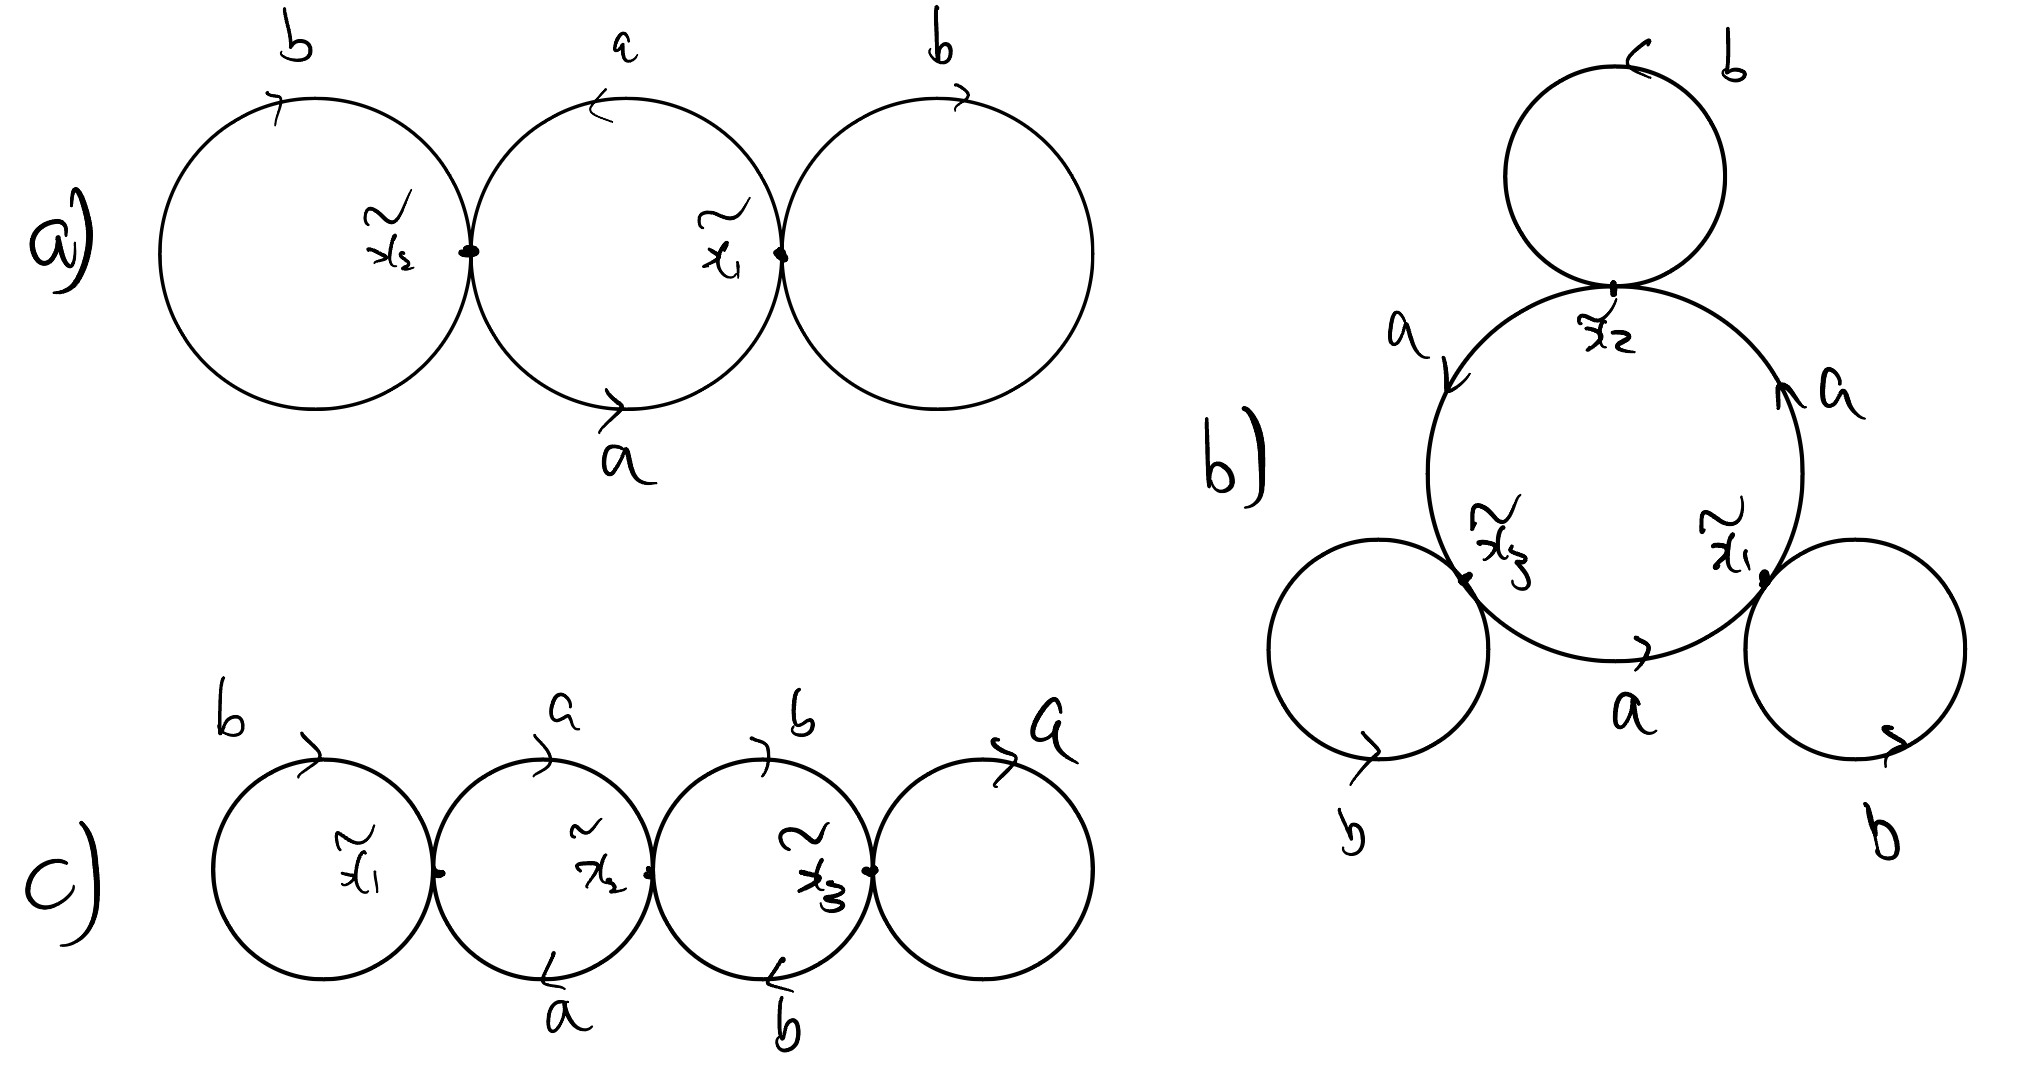
\includegraphics[width=0.8\textwidth]{./figures/monodromy.png}
	\caption{monodromy.png}
\end{figure}
~\begin{enumerate}[label=(\alph*)]
	\item $ a \mapsto (12),b\mapsto \text{id}$.
	\item $ a\mapsto (123), b \mapsto \text{id}$.
	\item $ a\mapsto (12), b \mapsto (23)$.
\end{enumerate}
\end{problem}

\begin{problem}[13]
Given $ f:X \to S^{1}$, since $ \pi_1( X) $ is finite, $ f_*( \pi_1( X) )$ is also finite, and the only finite subgroup of $ \pi_1( S^{1}) \cong \zz$ is the trivial subgroup. Thus $ f_*( \pi_1( X) ) = 0 = p_*( \pi_1( \rr) )$, satisfying the lifting criterion. Thus we have a lift $ \widetilde{ f}: X \to \rr$. Since $ \rr$ is contractible, $ \widetilde{ f}$ is nullhomotopic upstairs via $ \widetilde{ H}$, and $ f$ is nullhomotopic downstairs via  $ p \circ \widetilde{ H}$.
\end{problem}
\end{document}
